\documentclass[a4paper,11pt]{article}
% Use ctrl + alt + V to view live pdf

% Packages
\usepackage[utf8]{inputenc} % For encoding
\usepackage[T1]{fontenc} % Better handling of accented characters and hyphenation
\usepackage{microtype} % Improves spacing and justification
\usepackage{amsmath, amssymb} % For equations and symbols
\usepackage{graphicx} % For including graphics/images
\usepackage{caption} % For customizing figure and table captions
\usepackage{subcaption} % For subfigures and subcaptions
\usepackage{float} % For fixing figure and table positions
\usepackage{booktabs} % For professional-looking tables
\usepackage{siunitx} % For consistent typesetting of units and numbers
\usepackage[margin=2cm]{geometry} % Adjusts page margins
\usepackage{fancyhdr} % For custom headers and footers
\usepackage{lmodern} % For a professional-looking font (main body font)
\usepackage{titlesec} % For title customization
\usepackage{array} % For custom table formatting
\usepackage[colorlinks=true, linkcolor=black, urlcolor=black]{hyperref} % Colored links without boxes
\usepackage{cleveref} % For improved cross-referencing    
\usepackage{multirow}
\usepackage{enumitem}
\usepackage{listings}
\usepackage{xcolor}
\usepackage{textcomp}
\usepackage{tabularx}
\usepackage{changepage}
\usepackage{tikz}
\usepackage{pdfpages}
\usepackage[table]{xcolor}
\usetikzlibrary{shapes.geometric, arrows}
% --- C++ Style ---
\lstdefinestyle{cpp-style}{
    language=C++,
    basicstyle=\ttfamily\footnotesize,
    keywordstyle=\color{blue}\bfseries,
    stringstyle=\color{orange},
    commentstyle=\color{gray}\itshape,
    numbers=left,
    numberstyle=\tiny\color{gray},
    numbersep=10pt,
    backgroundcolor=\color{white},
    showspaces=false,
    showstringspaces=false,
    breaklines=true,
    breakatwhitespace=true,
    tabsize=4,
    captionpos=b,
    frame=single,
    rulecolor=\color{black},
}

% --- Python Style ---
\lstdefinestyle{python-style}{
    language=Python,
    basicstyle=\ttfamily\footnotesize,
    keywordstyle=\color{blue}\bfseries,
    commentstyle=\color{gray}\itshape,
    stringstyle=\color{green!50!black},
    frame=single,
    breaklines=true,
    showstringspaces=false,
    captionpos=b
}
\renewcommand{\lstlistingname}{Code}
% Custom settings
\pagestyle{fancy}
\fancyhf{}
\fancyhead[L]{\textit{SF4 - DataLogger}} % Header left
\fancyhead[R]{\textit{Will Hewes - wh365}} % Header right 
\fancyfoot[C]{\thepage} % Footer center
\setlength{\headheight}{15pt} % Header height
\setlength{\parindent}{0em} % Indentation for paragraphs
\setlength{\parskip}{0.5em} % Add spacing between paragraphs
\setlength{\abovedisplayskip}{1em}
\setlength{\belowdisplayskip}{1em}
\setlength{\abovedisplayshortskip}{1em}
\setlength{\belowdisplayshortskip}{1em}
% \setlist{topsep=0.2em, partopsep=0em, itemsep=0.1em, parsep=0em}

\graphicspath{{Images/}}

% \renewcommand{\arraystretch}{1.2}

% Title formatting
\renewcommand{\maketitle}{
    \begin{center}
        \LARGE \textbf{ENGINEERING TRIPOS PART IIA} \\[0.5em]
        \Large \textbf{SF4 - DataLogger} \\[0.5em]
        \textbf{Final Report} \\[1.5em]
        \vspace{-1em}
        \small Will Hewes - wh365 \\ 
        Pembroke College \\ 
        \vspace{0.5em}
    \end{center}
}

\begin{document}
\pagenumbering{gobble}
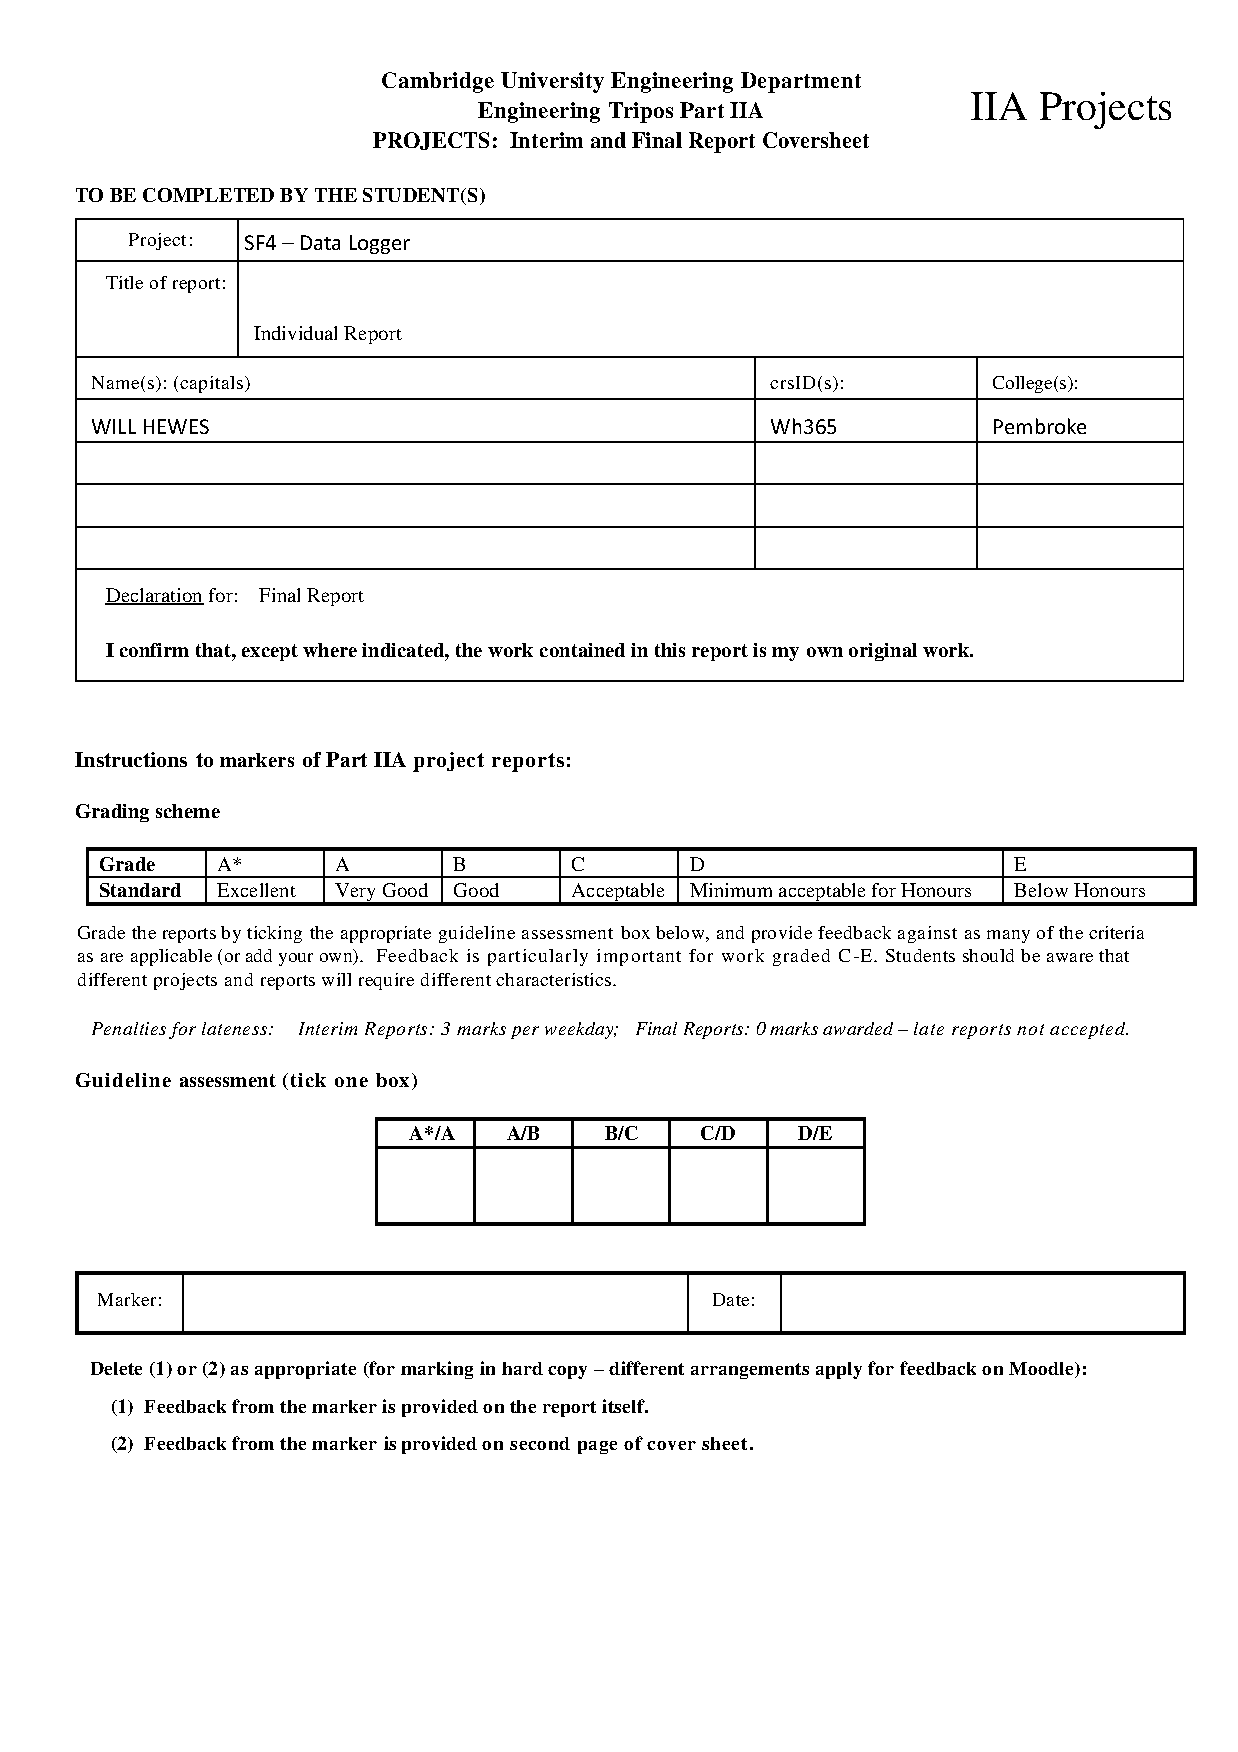
\includepdf[pages=-]{Handouts/IIA_Project_Coversheet Final Report.pdf}
\maketitle
\hrule
\tableofcontents
\newpage
\pagenumbering{arabic} \setcounter{page}{1}

\section{Introduction}
\label{sec:Introduction}

The aim of this project was to develop a microcontroller-based 
automatic plant watering system.
The system can autonomously monitor soil moisture levels, 
plot the data over time, and provide options to water the plant
at scheduled intervals or in response to threshold moisture levels.
This allows for effective monitoring and care with minimal user intervention.

In addition to moisture sensing, the system also tracks temperature, 
and was supposed to track humidity and light 
but our components did not arrive in time.
This means most of the key factors affecting plant health
can be closely tracked, enabling detailed analysis of
optimum conditions for plant health.
These additional features enhance the system's utility
for control and research.

The motivation behind creating this autonomous watering system was twofold. 
Firstly, it can be used as demonstrated on a small scale,
allowing direct control over the health of one 
or a small number of houseplants. 
This will remove the mamjority of the care required
to look after these often frail plants,
which is particularly useful over holidays or 
during the hot Summer months.
As a universty student with several well-loved plants,
this is very appealing to me personally
and I will in all likelihood implement this 
for my personal use once the project is finished.
Secondly, it provides an easily expandable system
which could be integrated into industrial applications.
There have been attempts to spread similar technologies 
throughout various industries, 
including the agrcultural industry where crop health 
and harvest timing are crucial. 
Some of these applications are discussed further in
Section \ref{sec:Further_Improvements}.

\section{Summary}
\label{sec:Summary}
% Summary of overall design decisions and outline of project management (1 side, possible team material)
- hosted on Github for collaboration \\
- outline timescale and plans for milestones\\
- building initial circuitry\\
- block diagram\\
- working submodules and testing equipment before integration\\
- decision for Tkinter, GUI etc.\\
- implementation of the socket demonstration before moving over to serial comms \\
- what processing would be done on PC vs on Arduino (future expansion to wifi / bluetooth)\\
- decisions behind including sensor types \\
- contruction of water delivery mechanism\\
- ordering parts through Farnell

\begin{table}[H]
    \centering
    \renewcommand{\arraystretch}{1.5} 
    \makebox[\linewidth][c]{
    \resizebox{0.8\textwidth}{!}{
    \begin{tabular}{|c|c|c|}
        \hline
        \textbf{Order Code} & \textbf{Description of Component} & \textbf{Unit Price (£)} \\
        \hline
        2946124 & Capacitive Soil Moisture Sensor Module & 4.69 \\
        \hline
        SC21096 & Mini servo & 2.94 \\
        \hline
        4030054 & Temperature sensor & 1.38 \\
        \hline
        \rowcolor{yellow!60} 3167525 & Light sensor & 1.43 \\
        \hline
        \rowcolor{yellow!60} SN36746 & Humidity sensor & 0.91 \\
        \hline
        \multicolumn{2}{|c|}{\textbf{\large Total}} & \textbf{\large 11.35} \\
        \hline
    \end{tabular}
    }   
    }
    \caption{Component Order Summary}
    \label{tab:component_order}
\end{table}

\section{System Architecture}
\label{sec:System_Architecture}
% Include anmalogue circuitry, block diagram, and decision to include capacitors, lack of resistors etc.
% External power supply for servo

- block diagram\\
- description of general structure

\begin{figure}[H]
    \centering
    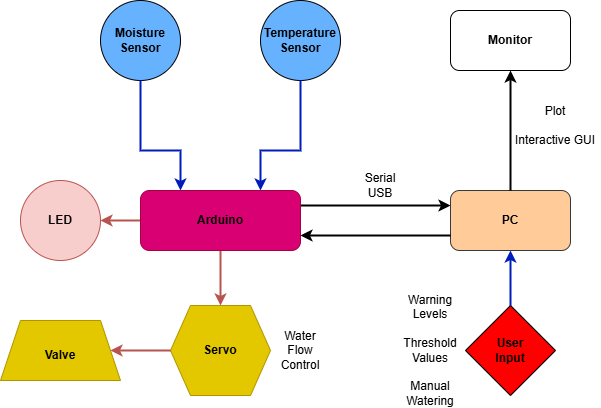
\includegraphics[width=0.8\textwidth]{Datalogger Block Diagram - final.png}
    \caption{Block Diagram for the automatic watering system}
    \label{fig:Block_Diagram_for_the_automatic_watering_system}
\end{figure}

\subsection{Circuit Design}
\label{Cicuit_Design}

- diagram\\
- testing sensors\\
- servo on seperate rail\\ 
- need for capacitors

\begin{figure}[H]
    \centering
    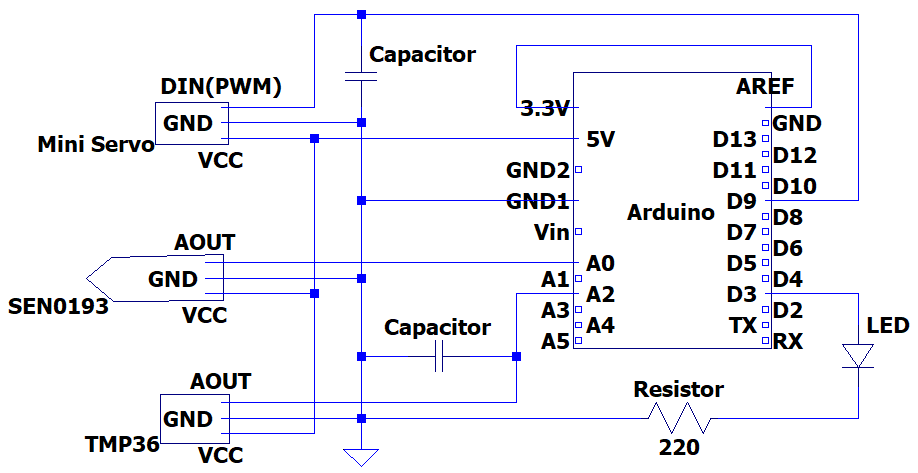
\includegraphics[width=0.8\textwidth]{Analogue Circuit Diagram - final.png}
    \caption{Analogue Circuit Diagram for the automatic watering system}
    \label{fig:Analogue_Circuit_Diagram_for_the_automatic_watering_system}
\end{figure}

\subsection{Watering System}
\label{sec:Watering_System}

- decision to use pinch valve\\
- necessity of reservoir sensor\\ 
- demonstration of components individually and collectively

\section{Code}
\label{sec:Code}
% Description of design/ computer code
\subsection{Firmware}
\label{sec:Firmware}
- sensors\\
- parsing, processing\\
- servo control

\subsection{Software}
\label{sec:Software}
- comms with Arduino\\
- GUI, plotting\\
- initial demonstration

\section{Technical Problemms}
\label{sec:Technical_Problems}
% Outline problems encountered in development and their technical solutions
- get Chengs help in drafting some interesting ones \\
- outline problem with powerrail if appropriate (not realising that these breadboards come with a gap in the powerrail)\\
- floating point problem for temp sensor

\section{Test Procedure}
\label{sec:Test_Procedure}
% Test procedure and software implementation
- testing individual compomnents one at a time \\
- testing the software presentation with a demonstration random data supply\\
- calibrating the moisture sensor with dry and with water\\
- determining the required servo rotation to elicit small quanmtiy of water\\
- use data from other sources to determine if humidity, light, and temp calibrated properly

\section{Further Improvements}
\label{sec:Further_Improvements}
- wifi module \\
- less jerryrigged water supply\\
- more sensors (CO2 conc)\\
- reservoir sensor\\
- greater control over parameters (mass of plant, type of plant)\\
- greater signal processing\\
- wider industrial applications

\subsection{Wider Industry}
\label{sec:Wider_Industry}
% Mention the watering systems currently being developed and the research undertaken
- deeper research into exact requirements\\
- close collaboration with farmers to set these requirements\\
- integrate a warning system to say that the specific conditions have been met (humidity requirements for harvesting etc, perhaps dangerous levels of heat)\\
- further integration of sensors, such as soil content (salt conc, fertiliser etc.)

\section{Conclusion}
\label{sec:Conclusion}

The aim of this project was to create a working demonstration of 
our autonomous watering system, with the ability to both log data
and dispense controlled quantities of water 
as the consumer dictates.
Overall, this has been a resounding success, 
acheiving the inital goal of moisture sensing and servo activation,
and expanding on this to include other senors 
and a more developed GUI.

The primary challenges and takeaways for a similar project in the future
include ...
Throughout this report it is evident that responsible practises 
such as detailed planning, modular testing,
and a feasible but expandable scope are integral to 
ensuring the success of a project like this.

This work could be expanded in the future to make a 
more sophisticated and professional datalogger
of the same scale,
incorporating more sensors, a more ... housing and 
general setup,
or could be further modified to be used in larger
industrial applications, such as informing agricultural farming
as is being researched by ...

\newpage
\appendix
\begin{thebibliography}{9}

\bibitem{arduino_servo}
Arduino. \textit{Servo Motor Basics with Arduino} : \\
\url{https://docs.arduino.cc/learn/electronics/servo-motors/}

\bibitem{tmp36}
Analog Devices. \textit{TMP35/TMP36/TMP37 Data Sheet} : \\
\url{https://www.analog.com/en/products/tmp36.html} 

\bibitem{arduino_tmp36}
ArduinoGetStarted. \textit{Arduino - TMP36 Temperature Sensor} : \\
\url{https://arduinogetstarted.com/tutorials/arduino-tmp36-temperature-sensor}

\bibitem{dfrobot}
DFRobot. \textit{Capacitive Soil Moisture Sensor SKU SEN0193} : \\
\url{https://wiki.dfrobot.com/Capacitive_Soil_Moisture_Sensor_SKU_SEN0193}

\bibitem{yt}
YouTube. \textit{Improving Capacitive Soil Moisture Sensor Readings} : \\
\url{https://youtu.be/QGCrtXf8YSs}

\bibitem{pinch_valve_design}
Printables. \textit{Pinch Valve Powered by Servo} : \\
\url{https://www.printables.com/model/247744-pinch-valve-powered-by-servo/files}

\end{thebibliography}

\section{Interim Report}
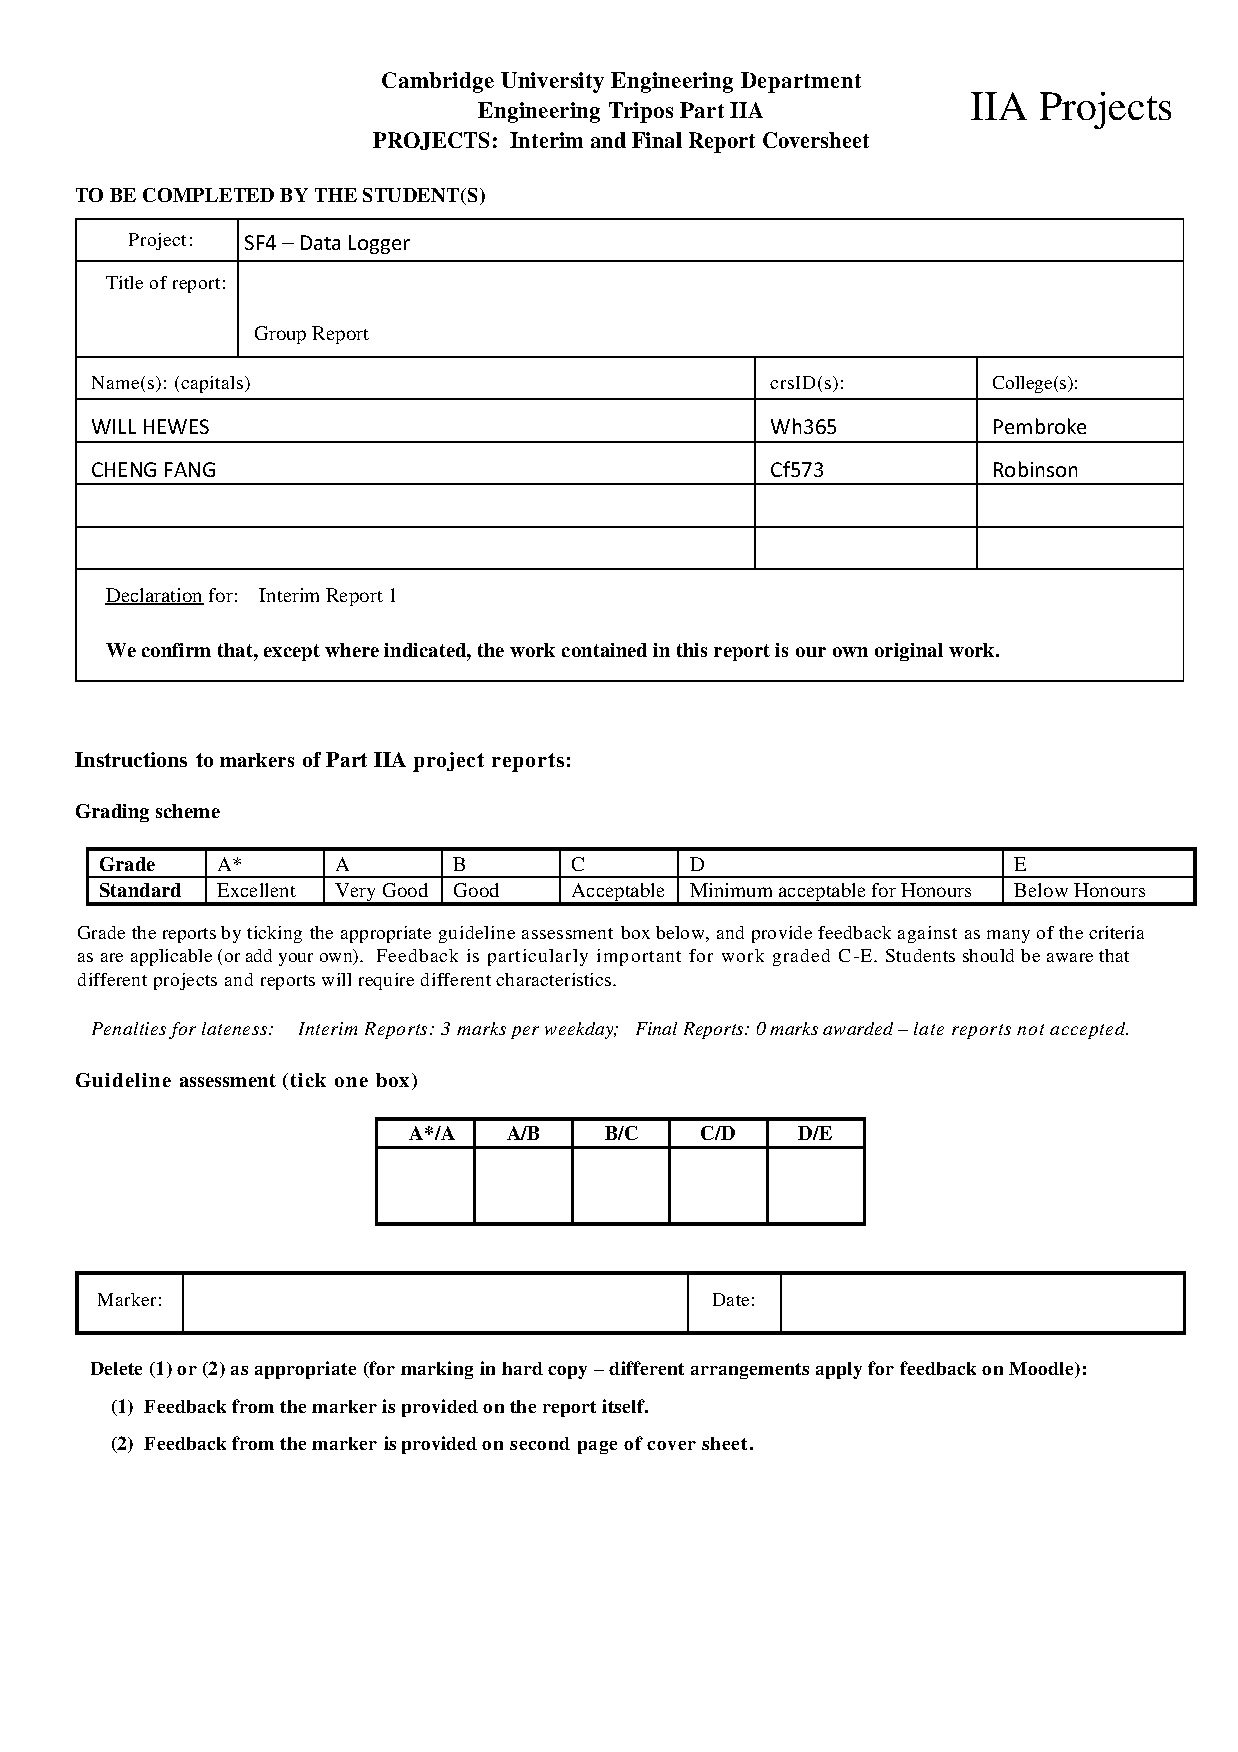
\includepdf[pages=-]{Reports/First Interim Report.pdf} % e.g. [pages={1,3-5,7}] to include pages 1,3,4,5,7
% Featuring the Interim Report

\end{document}